\section{Financial\_\-Monthly\_\-Category  Class Reference}
\label{classFinancial__Monthly__Category}\index{Financial_Monthly_Category@{Financial\_\-Monthly\_\-Category}}
{\tt \#include $<$dil2al.hh$>$}

Inheritance diagram for Financial\_\-Monthly\_\-Category::\begin{figure}[H]
\begin{center}
\leavevmode
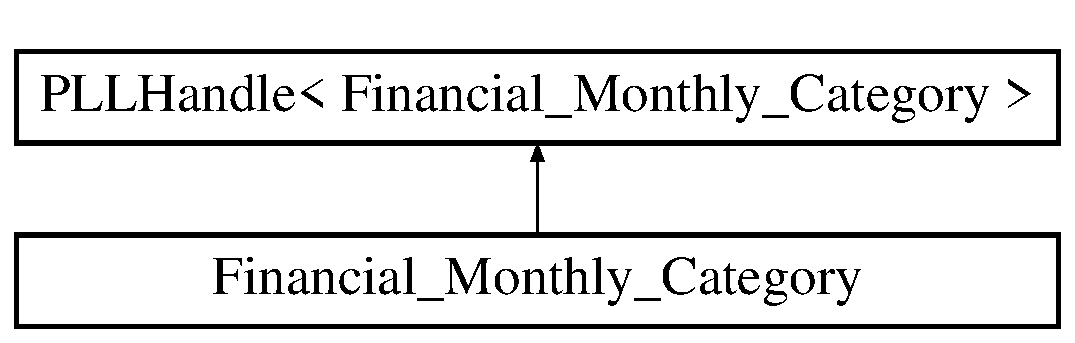
\includegraphics[height=2cm]{classFinancial__Monthly__Category}
\end{center}
\end{figure}
\subsection*{Public Methods}
\begin{CompactItemize}
\item 
{\bf Financial\_\-Monthly\_\-Category} ({\bf String} c, double r=0.0)
\item 
{\bf String} {\bf Category} () const
\item 
Financial\_\-Monthly\_\-Category $\ast$ {\bf Find\_\-Category} ({\bf String} c) const
\item 
double {\bf Result} () const
\item 
void {\bf Copy\_\-Sub\-Categories} (Financial\_\-Monthly\_\-Category $\ast$c)
\item 
void {\bf add} ({\bf String} s, double e, {\bf Financial\_\-Monthly} \&month)
\end{CompactItemize}
\subsection*{Public Attributes}
\begin{CompactItemize}
\item 
{\bf PLLRoot}$<$ {\bf Financial\_\-Monthly\_\-Sub\-Category} $>$ {\bf subcategories}
\end{CompactItemize}
\subsection*{Protected Attributes}
\begin{CompactItemize}
\item 
{\bf String} {\bf category}
\item 
double {\bf result}
\end{CompactItemize}


\subsection{Constructor \& Destructor Documentation}
\index{Financial_Monthly_Category@{Financial\_\-Monthly\_\-Category}!Financial_Monthly_Category@{Financial\_\-Monthly\_\-Category}}
\index{Financial_Monthly_Category@{Financial\_\-Monthly\_\-Category}!Financial_Monthly_Category@{Financial\_\-Monthly\_\-Category}}
\subsubsection{\setlength{\rightskip}{0pt plus 5cm}Financial\_\-Monthly\_\-Category::Financial\_\-Monthly\_\-Category ({\bf String} {\em c}, double {\em r} = 0.0)\hspace{0.3cm}{\tt  [inline]}}\label{classFinancial__Monthly__Category_a0}




Definition at line 1121 of file dil2al.hh.

References result.



\footnotesize\begin{verbatim}1121 : category(c), result(r) {}
\end{verbatim}\normalsize 


\subsection{Member Function Documentation}
\index{Financial_Monthly_Category@{Financial\_\-Monthly\_\-Category}!add@{add}}
\index{add@{add}!Financial_Monthly_Category@{Financial\_\-Monthly\_\-Category}}
\subsubsection{\setlength{\rightskip}{0pt plus 5cm}void Financial\_\-Monthly\_\-Category::add ({\bf String} {\em s}, double {\em e}, {\bf Financial\_\-Monthly} \& {\em month})}\label{classFinancial__Monthly__Category_a5}




Definition at line 175 of file finances.cc.

References Financial\_\-Monthly\_\-Sub\-Category::add(), category, Financial\_\-Monthly\_\-Sub\-Category::Find\_\-Sub\-Category(), PLLHandle$<$ Financial\_\-Monthly $>$::head(), PLLRoot$<$ Financial\_\-Monthly\_\-Sub\-Category $>$::head(), String::index(), PLLRoot$<$ Financial\_\-Monthly\_\-Sub\-Category $>$::link\_\-before(), PLL\_\-LOOP\_\-FORWARD, result, String::sub(), subcategories, and PLLRoot$<$ Financial\_\-Monthly\_\-Sub\-Category $>$::tail().

Referenced by Financial\_\-Monthly::add().



\footnotesize\begin{verbatim}175                                                                                   {
176   // add to result and by subcategory
177   result += e;
178   if (s.index(BRXidentifier)<0) s = "general";
179   else s = s.sub(BRXidentifier,0);
180   Financial_Monthly_SubCategory * fs = NULL;
181   if (subcategories.head()) fs = subcategories.head()->Find_SubCategory(s);
182   if (!fs) { // add subcategory in this category in all months
183     PLL_LOOP_FORWARD(Financial_Monthly,month.head(),1) {
184       Financial_Monthly_Category * fc = e->categories.head()->Find_Category(category);
185       fs = new Financial_Monthly_SubCategory(s);
186       fc->subcategories.link_before(fs);
187     }
188     fs = subcategories.tail(); // retrieve subcategory in this month and category
189   }
190   // add to subcategory result
191   fs->add(e);
192 }
\end{verbatim}\normalsize 
\index{Financial_Monthly_Category@{Financial\_\-Monthly\_\-Category}!Category@{Category}}
\index{Category@{Category}!Financial_Monthly_Category@{Financial\_\-Monthly\_\-Category}}
\subsubsection{\setlength{\rightskip}{0pt plus 5cm}{\bf String} Financial\_\-Monthly\_\-Category::Category () const\hspace{0.3cm}{\tt  [inline]}}\label{classFinancial__Monthly__Category_a1}




Definition at line 1123 of file dil2al.hh.



\footnotesize\begin{verbatim}1123 { return category; }
\end{verbatim}\normalsize 
\index{Financial_Monthly_Category@{Financial\_\-Monthly\_\-Category}!Copy_SubCategories@{Copy\_\-SubCategories}}
\index{Copy_SubCategories@{Copy\_\-SubCategories}!Financial_Monthly_Category@{Financial\_\-Monthly\_\-Category}}
\subsubsection{\setlength{\rightskip}{0pt plus 5cm}void Financial\_\-Monthly\_\-Category::Copy\_\-Sub\-Categories (Financial\_\-Monthly\_\-Category $\ast$ {\em c})}\label{classFinancial__Monthly__Category_a4}




Definition at line 167 of file finances.cc.

References PLLRoot$<$ Financial\_\-Monthly\_\-Sub\-Category $>$::head(), PLLRoot$<$ Financial\_\-Monthly\_\-Sub\-Category $>$::link\_\-before(), PLL\_\-LOOP\_\-FORWARD, and subcategories.

Referenced by Financial\_\-Monthly::Copy\_\-Categories().



\footnotesize\begin{verbatim}167                                                                                   {
168   if (c==this) return; // no other category to copy from
169   PLL_LOOP_FORWARD(Financial_Monthly_SubCategory,c->subcategories.head(),1) {
170     Financial_Monthly_SubCategory * fs = new Financial_Monthly_SubCategory(e->SubCategory());
171     subcategories.link_before(fs);
172   }
173 }
\end{verbatim}\normalsize 
\index{Financial_Monthly_Category@{Financial\_\-Monthly\_\-Category}!Find_Category@{Find\_\-Category}}
\index{Find_Category@{Find\_\-Category}!Financial_Monthly_Category@{Financial\_\-Monthly\_\-Category}}
\subsubsection{\setlength{\rightskip}{0pt plus 5cm}Financial\_\-Monthly\_\-Category $\ast$ Financial\_\-Monthly\_\-Category::Find\_\-Category ({\bf String} {\em c}) const}\label{classFinancial__Monthly__Category_a2}




Definition at line 161 of file finances.cc.

References category, and PLLHandle$<$ Financial\_\-Monthly\_\-Category $>$::Next().

Referenced by Financial\_\-Monthly::add().



\footnotesize\begin{verbatim}161                                                                                      {
162   if (category==c) return const_cast<Financial_Monthly_Category *>(this);
163   if (Next()) return Next()->Find_Category(c);
164   return NULL;
165 }
\end{verbatim}\normalsize 
\index{Financial_Monthly_Category@{Financial\_\-Monthly\_\-Category}!Result@{Result}}
\index{Result@{Result}!Financial_Monthly_Category@{Financial\_\-Monthly\_\-Category}}
\subsubsection{\setlength{\rightskip}{0pt plus 5cm}double Financial\_\-Monthly\_\-Category::Result () const\hspace{0.3cm}{\tt  [inline]}}\label{classFinancial__Monthly__Category_a3}




Definition at line 1125 of file dil2al.hh.

References result.



\footnotesize\begin{verbatim}1125 { return result; }
\end{verbatim}\normalsize 


\subsection{Member Data Documentation}
\index{Financial_Monthly_Category@{Financial\_\-Monthly\_\-Category}!category@{category}}
\index{category@{category}!Financial_Monthly_Category@{Financial\_\-Monthly\_\-Category}}
\subsubsection{\setlength{\rightskip}{0pt plus 5cm}{\bf String} Financial\_\-Monthly\_\-Category::category\hspace{0.3cm}{\tt  [protected]}}\label{classFinancial__Monthly__Category_n0}




Definition at line 1118 of file dil2al.hh.

Referenced by add(), and Find\_\-Category().\index{Financial_Monthly_Category@{Financial\_\-Monthly\_\-Category}!result@{result}}
\index{result@{result}!Financial_Monthly_Category@{Financial\_\-Monthly\_\-Category}}
\subsubsection{\setlength{\rightskip}{0pt plus 5cm}double Financial\_\-Monthly\_\-Category::result\hspace{0.3cm}{\tt  [protected]}}\label{classFinancial__Monthly__Category_n1}




Definition at line 1119 of file dil2al.hh.

Referenced by add(), Financial\_\-Monthly\_\-Category(), and Result().\index{Financial_Monthly_Category@{Financial\_\-Monthly\_\-Category}!subcategories@{subcategories}}
\index{subcategories@{subcategories}!Financial_Monthly_Category@{Financial\_\-Monthly\_\-Category}}
\subsubsection{\setlength{\rightskip}{0pt plus 5cm}{\bf PLLRoot}$<${\bf Financial\_\-Monthly\_\-Sub\-Category}$>$ Financial\_\-Monthly\_\-Category::subcategories}\label{classFinancial__Monthly__Category_m0}




Definition at line 1122 of file dil2al.hh.

Referenced by add(), and Copy\_\-Sub\-Categories().

The documentation for this class was generated from the following files:\begin{CompactItemize}
\item 
{\bf dil2al.hh}\item 
{\bf finances.cc}\end{CompactItemize}
